\documentclass[11pt]{beamer}
\usepackage[utf8]{inputenc}
\usepackage[T1]{fontenc}
\usepackage{transparent}
\usepackage[backend=bibtex,style=authoryear]{biblatex}
\addbibresource{brownbags.bib}

%% End of citations additions

%\usetheme{AnnArbor}
%\usetheme{Antibes}
%\usetheme{Berkeley}
%\usetheme{Berlin}
%\usetheme{boxes}
%\usetheme{Darmstadt}
%\usetheme{default}
%\usetheme{Frankfurt}
%\usetheme{Ilmenau}
%\usetheme{JuanLesPins}
\usetheme{Luebeck}
%\usetheme{Malmoe}
%\usetheme{Montpellier}
%\usetheme{PaloAlto}
%\usetheme{Rochester}
%\usetheme{Singapore}
%\usetheme{Szeged}
%\hypersetup{
%	colorlinks=true,
%	linkcolor=blue,
%	filecolor=magenta,      
%	urlcolor=cyan,
%}

\setbeamertemplate{footline}
{%
	\leavevmode%
	\hbox{\begin{beamercolorbox}[wd=.2\paperwidth,ht=2.5ex,dp=1.125ex,leftskip=.3cm,rightskip=.3cm plus1fill]{author in head/foot}%
			\usebeamerfont{author in head/foot} \insertframenumber{} / \inserttotalframenumber
		\end{beamercolorbox}%
		\begin{beamercolorbox}[wd=.3\paperwidth,ht=2.5ex,dp=1.125ex,leftskip=.3cm plus1fill,rightskip=.3cm]{author in head/foot}%
			\usebeamerfont{author in head/foot}\insertshortauthor
		\end{beamercolorbox}%
		\begin{beamercolorbox}[wd=.5\paperwidth,ht=2.5ex,dp=1.125ex,leftskip=.3cm,rightskip=.3cm plus1fil]{title in head/foot}%
			\usebeamerfont{title in head/foot}\insertshorttitle
	\end{beamercolorbox}}%
	\vskip0pt%
}
\setbeamertemplate{headline}{}

\begin{document}
	\author{Gary R Seamans}
	\title{Machine Learning}
	\subtitle{R Brown Bag Series \#6}
	%\logo{\scalebox{0.035}{
\includegraphics{R_logo.png}}}
	\institute{The MITRE Corporation}
	%\date{}
	%\subject{}
	%\setbeamercovered{transparent}
	%\setbeamertemplate{navigation symbols}{}
	\begin{frame}[plain]
		\maketitle
    \end{frame}

\begin{frame}{
	\begin{minipage}[t]{0.55\textwidth}
		Agenda
	\end{minipage}
	\hfill
	\begin{minipage}[t]{0.35\textwidth}
		\flushright
		\scalebox{0.035}{
\includegraphics{R_logo.png}}
	\end{minipage}
}{}
%% ==================== Content ===========================%%
\begin{center}
	\begin{itemize}
		\item Definition
		\item ML Techniques and Categories
		\item Examples
		\item Discussions
	\end{itemize}
\end{center}
\end{frame}

\usebackgroundtemplate{\transparent{0.4}
\includegraphics[width=\paperwidth, 
	height=\paperheight]{Machine-Learning.png}}
%% Definition ===================
\begin{frame}{
	\begin{minipage}[t]{0.55\textwidth}
		Definition
	\end{minipage}
	\hfill
	\begin{minipage}[t]{0.35\textwidth}
		\flushright
		\scalebox{0.035}{
\includegraphics{R_logo.png}}
	\end{minipage}
}{}
%% ==================== Content ===========================%%
What is machine learning?

\begin{center}
	\textit{“Machine Learning is the science of getting computers to learn and act like humans do, and improve their learning over time in autonomous fashion, by feeding them data and information in the form of observations and real-world interactions.”}\cite{ml2018}
\end{center}

\end{frame}
\usebackgroundtemplate{}
%% Common Techniques ===================
\begin{frame}{
	\begin{minipage}[t]{0.55\textwidth}
		Common ML Techniques
	\end{minipage}
	\hfill
	\begin{minipage}[t]{0.35\textwidth}
		\flushright
		\scalebox{0.035}{
\includegraphics{R_logo.png}}
	\end{minipage}
}{}
%% ==================== Content ===========================%%

\begin{center}
	\textbf{ML Categories}
	\begin{itemize}
		\item Supervised Machine Learning
		\item Unsupervised Machine Learning
		\item Reinforcement Machine Learning
	\end{itemize}
\end{center}
\begin{center}
	\textbf{ML Techniques}
	\begin{columns}
		\begin{column}[t]{0.45\textwidth}
			\begin{itemize}
				\item Naïve Bayes Classifier
				\item K Means Clustering
				\item Support Vector Machine
				\item Apriori 
				\item Linear Regression
			\end{itemize}
		\end{column}
		\begin{column}[t]{0.45\textwidth}
			\begin{itemize}
				\item Logistic Regression
				\item Artificial Neural Networks
				\item Random Forests
				\item Decision Trees
				\item Nearest Neighbours
			\end{itemize}
		\end{column}
	\end{columns}
\end{center}
\cite{Top10Machine}
\end{frame}

%% Cancer Example ===================
\begin{frame}{
	\begin{minipage}[t]{0.55\textwidth}
		Cancer Example
	\end{minipage}
	\hfill
	\begin{minipage}[t]{0.35\textwidth}
		\flushright
		\scalebox{0.035}{
\includegraphics{R_logo.png}}
	\end{minipage}
}{}
%% ==================== Content ===========================%%

This example uses decision trees to determine tumor spread.
\begin{itemize}
	\item Predicts tumor spread in this dataset of 97 men who had undergone a biopsy.
	\item Measures used for prediction: BPH, PSA, Gleason Score, CP, and size of prostate.
\end{itemize}
\end{frame}

%% Exercise  ===================
\begin{frame}{
	\begin{minipage}[t]{0.55\textwidth}
		Exercise type
	\end{minipage}
	\hfill
	\begin{minipage}[t]{0.35\textwidth}
		\flushright
		\scalebox{0.035}{
\includegraphics{R_logo.png}}
	\end{minipage}
}{}
%% ==================== Content ===========================%%
The goal is to use data from accelerometers on the belt, forearm, arm, and dumbell of 6 participants to predict the manner in which the participants did each exercise.  

\vspace{0.5cm}
Three different methods were used: - Random Forests - Naive Bayes - Boosting with trees (gbm)
\end{frame}



%% Extra Links ===================
\begin{frame}{
	\begin{minipage}[t]{0.55\textwidth}
		Extra Resources
	\end{minipage}
	\hfill
	\begin{minipage}[t]{0.35\textwidth}
		\flushright
		\scalebox{0.035}{
\includegraphics{R_logo.png}}
	\end{minipage}
}{}
%% ==================== Content ===========================%%
\begin{itemize}
	\item \href{http://topepo.github.io/caret/index.html}{The \textbf{caret} package}
	\item \href{https://lgatto.github.io/IntroMachineLearningWithR/an-introduction-to-machine-learning-with-r.html}{Introduction to Machine Learning with R}
	\item \href{https://www.r-bloggers.com/in-depth-introduction-to-machine-learning-in-15-hours-of-expert-videos/}{In-depth introduction to machine learning in 15 hours of expert videos}
	\item \href{EnsemblesAndRandomForest.pdf}{Short discussion on Ensembles and Random Forests}
\end{itemize}
\end{frame}

\usebackgroundtemplate{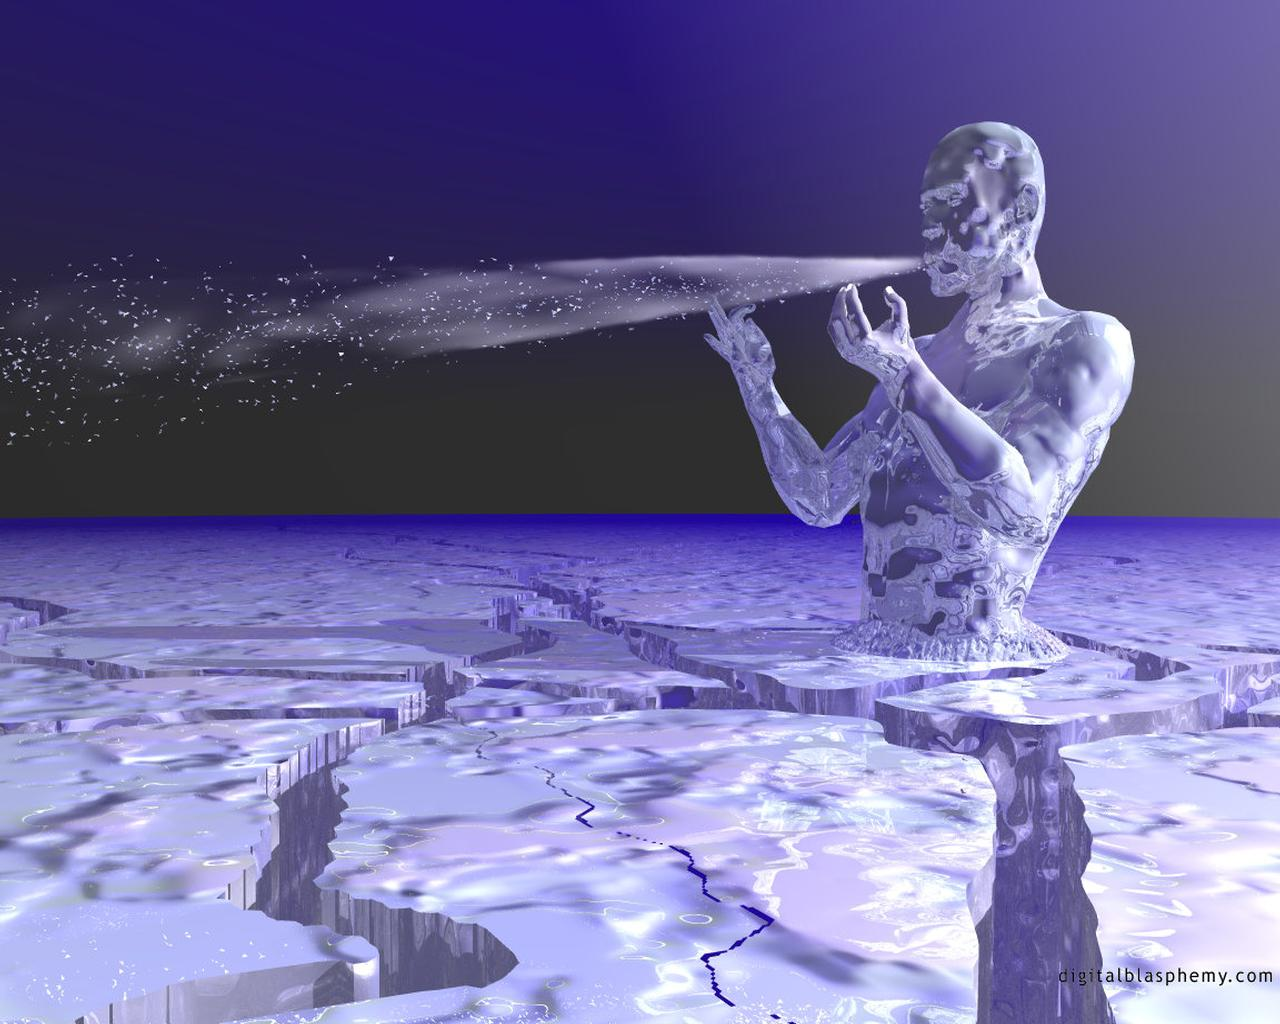
\includegraphics[width=\paperwidth, height=\paperheight]{frio_1280.jpg}}
%% Questions ===================
\begin{frame}{
	\begin{minipage}[t]{0.55\textwidth}
		Questions
	\end{minipage}
	\hfill
	\begin{minipage}[t]{0.35\textwidth}
		\flushright
		\scalebox{0.035}{
\includegraphics{R_logo.png}}
	\end{minipage}
}{}
%% ==================== Content ===========================%%

\end{frame}

\usebackgroundtemplate{}

%%===================== Citations =================================%%
\appendix
\begin{frame}[allowframebreaks]{References}{}
\footnotesize
\printbibliography

\end{frame}
\end{document}